\chapter{Background}
\section{Virtualization}

The main task of any operating system is to basically manage the following four - physical - resources: Processor (CPU), Memory (RAM), Storage (HDD / SSD), The network card (NIC). The part of the operating system that does this and acts like a bridge between application and hardware of the computer is called the kernel. The means which a computer program uses, in order to request a service from the kernel of the operating system it is executed on, is called system calls (syscalls).

\begin{figure}[h!]
  \centering
   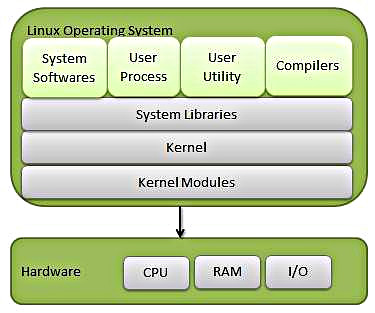
\includegraphics[width=0.45\linewidth]{./figures/linuxos.jpeg}
   \caption{Linux Operating System connecting to Hardware}
\end{figure}

Virtualization is technology that allows you to create multiple simulated environments or dedicated resources from a single, physical hardware system. \cite{redvirtual}

A software called a hypervisor, also referred to as Virtual Machine Manager (VMM), connects directly to that hardware and allows the host computer to share its resources from the hardware and distribute them appropriately between separate, distinct, and secure environments known as virtual machines (VMs). The physical hardware, equipped with a hypervisor, is called the host, while the many VMs that use its resources are guests.

There are two types of Hypervisors: \cite{dockerall}
\begin{description}[style=nextline]
\item[Type 1 or \say{Bare Metal Hypervisor}]

This software is installed right on top of the underlying machine's hardware (so, in this case, there is no host OS, there are only guest OS's). This type of hypervisors is encountered on machines on which the whole purpose is to run many virtual machines.

Type 1 hypervisors have their own device drivers and interact with hardware directly unlike type 2 hypervisors. That's what makes them faster, simpler and hence more stable.

Some examples of hypervisors of Type 1 are the following: VMware ESX and ESXi, Microsoft Hyper-V, Citrix XenServer, Oracle VM.

\item[Type 2 or \say{Hosted Hypervisor}]

This is a program that is installed on top of the operating system. This type of hypervisor is something like a \say{translator} that translates the guest operating system's system calls into the host operating system's system calls.

An upside of a Type 2 hypervisor is that in this case we don't have to worry about underlying hardware and its drivers. We really just need to delegate the job to the host OS, which will manage this stuff for us. The downside is that it creates a resource overhead, and multiple layers sitting on top of each other make things complicated and lowers the performance.

Some examples of hypervisors of Type 2 are the following: VMware Workstation/Fusion/Player, VMware Server, Microsoft Virtual PC, Oracle VM VirtualBox, Red Hat Enterprise Virtualization.
\end{description}
\begin{textblock*}{103cm}(7.6cm,17.1cm)
\textbf{Type 1}
\end{textblock*}
\begin{textblock*}{103cm}(12.4cm,17.1cm)
\textbf{Type 2}
\end{textblock*}
\begin{figure}[h!]
  \centering
   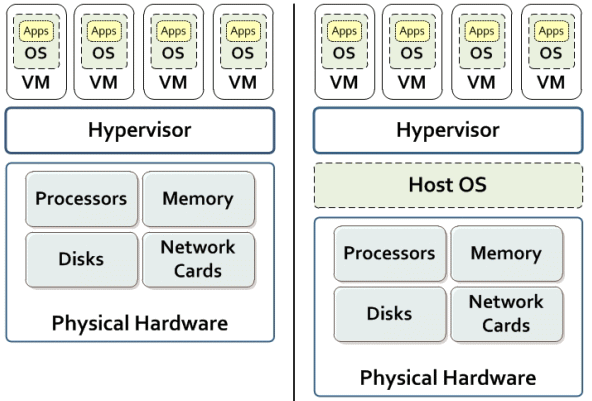
\includegraphics[width=0.6\linewidth]{./figures/hypervisors2.png}
   \caption{Hypervisor Type 1 and Hypervisor Type 2}
\end{figure}

\section{Docker}

\begin{figure}[h!]
  \centering
   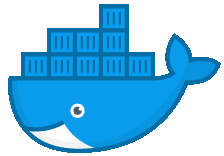
\includegraphics[width=0.3\linewidth]{./figures/Docker.png}
   \caption{Trademark of Docker}
\end{figure}

\subsection{What is Docker?}
Docker is a computer program that performs operating-system-level virtualization. It was first released in 2013 and is developed by Docker, Inc.

It is not a standalone software, but a platform to run and manage software packages called containers. It packages an application and all its dependencies together in the form of a docker container, in order to ensure that the application works seamlessly in any environment.

Containers had actually been the motivation for Docker's creation. Although they have been around for decades, Docker sought a way to make them easy to use, as it was a fact that people had already been very interested in Linux containers and how they could build something with them, but the problem was that Linux containers were very complicated. Docker's goal was achieved with great success and became the most popular container standard, as it made containers easier and safer to deploy and use, than previous approaches.

A docker container is a standard unit of software that packages up code and all its dependencies, so that the application runs quickly and reliably from one computing environment to another. A docker image is an executable package that includes everything needed to run an application (the code, a runtime, libraries, environment variables, configuration files) or, as it is commonly described, a read-only template used to build containers. The docker container is launched by running the docker image and is actually a runtime instance of the image, as it represents what the image becomes in memory when executed.

Some essential characteristics of docker containers and docker images are the following:
\begin{itemize}
\item Multiple containers, using the same image, can run at the same time sharing a single operating-system kernel, each running as isolated process in user space.
\item The limit of running containers is set by the number of processes that the hardware allows.
\item Whatever happens inside a container, does not affect the image it was made from.
\end{itemize}

Docker is mainly used by developers and sysadmins to develop, deploy, and run applications with containers. The use of Linux containers to deploy applications is called containerization.

Containerization is increasingly popular because containers are: \cite{dockergetstarted}
\begin{itemize}
\item Flexible: Even the most complex applications can be containerized.
\item Lightweight: Containers leverage and share the host kernel.
\item Interchangeable: You can deploy updates and upgrades on-the-fly.
\item Portable: You can build locally, deploy to the cloud, and run anywhere.
\item Scalable: You can increase and automatically distribute container replicas.
\item Stackable: You can stack services vertically and on-the-fly.
\end{itemize}

\subsection{Containerization vs Virtualization}

Containerization is not virtualization, as we described it in previous section, and Docker is definitely not a hypervisor. Containerization is the technique of bringing virtualization to the operating system level. While virtualization brings abstraction to the hardware, containerization brings abstraction to the operating system. \cite{conteintro} Therefore, containerization is more considered as a different kind of virtualization, known as operating-system-level virtualization or container-based virtualization.

Containers and virtual machines are only alike in the fact that they are both designed to provide an isolated environment, in which to run an application. Additionally, in both cases that environment is represented as a binary artifact that can be moved between hosts.

Apart from these similarities, containers and virtual machines are very different between each other and the key that lies on it is that the underlying architecture is fundamentally different between the two. More importantly, the fundamental goals of VMs and containers are different, as the purpose of a VM is to fully emulate a foreign environment, while the purpose of a container is to make applications portable and self-contained. \cite{bookdock}

Some of the advantages of Docker Containers over VMs are the following:
\begin{description}[style=nextline]
\item[Portability]
VMs have finite capabilities, because the hypervisors that create them are tied to the finite resources of a physical machine. Thus, if there are applications running in VMs, it is very difficult to migrate on another host environment. Containers, on the other hand, share the same operating system kernel and package applications with their runtime environments so the whole thing can be moved, opened, and used across development, testing, and production configurations. They provide the portability feature, as they are easily shipped or migrate from one environment to another.

\item[Resource management]
Once some resources are allocated for a VM, it's going to hold them as long as it's running. Moreover, VMs provide an environment with more resources than most applications need. On the other hand, containers do not waste physical resources, because they don't have a separate kernel, but they actually share resources with the host OS. Docker runs a discrete process as a container, taking no more memory than any other executable.

\item[Size and overhead]
All containers are run by a single operating-system kernel and are thus more lightweight than virtual machines. Moreover, while containers' images are typically tens of MBs in size, VMs usually take up tens of GBs. Hardware virtualization and virtual machines are extremely resource heavy. VMs end up taking a lot of RAM space and CPU cycles which ultimately incurs significant performance overhead.

\item[Boot up time]
Since the VM has its own kernel, when it comes to start-up or restart, operating system needs to start from scratch, which will then load all the binaries and libraries. This is time consuming and will prove very costly at times when quick startup of applications is needed.
On the other hand, in case of docker containers, boot up and restart happens very fast because they don't need to start up the kernel every time, since the container runs on the host OS.
\end{description}
\begin{figure}[h!]
  \centering
   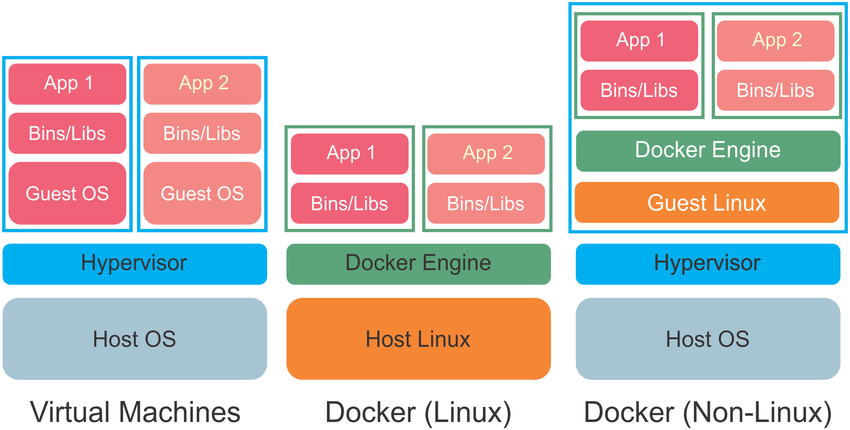
\includegraphics[width=0.75\linewidth]{./figures/vmdocklin.png}
   \caption{Virtual Machines vs Docker Containers on Linux and on other OS}
\end{figure}

The other side of the coin, though, is that there are also some drawbacks when choosing docker containers over VMs. Some of them are listed below:

\begin{description}[style=nextline]
\item[Identical host and guest kernel]
Virtual machines can use any OS as guest machine, not requiring for kernel of host and guest to be identical. However, in container-based virtualization, it is only possible to run containers of the same type as the underlying OS.  It is not possible to run Linux containers on Windows or Mac, because they need Linux kernel to operate. The solution for Mac and Windows users would be to install a hypervisor of Type 2, such as VirtualBox, boot up the Linux machine and then run Linux containers inside of it. This is exactly what Docker for Mac and Docker for Windows do, but they use native hypervisors that come with the respective OS. \cite{dockerall}

\item[Security]
The reason why virtual machines are considered to be more secure, is that containers make system calls directly to the kernel and a low-level software messing with a kernel directly could potentially lead to host machine getting cracked. This opens up a whole verity of vulnerabilities. On the other hand, in case of virtual machines, host and guest machines have the different kernels and are segregated from each other and thus, security is more prominent in case of virtual machines than containers. The one feature a VM usually has is that it is hardware isolated at the chip level through actual instructions: Intel VT-x or AMD-V. There are other ways for intruders to exploit you in these environments (such as rootkits) but they're much harder to install.

The main aspect of security that is at risk in containers is isolation, which is explicitly detailed in the next section while several types of attacks are described in \textit{Chapter 4}. Both VMs and containers can be used to isolate applications from other applications running on the same host. VMs have an added degree of isolation from the hypervisor and are a trusted and battle-hardened technology. Containers are comparatively new, and many organizations are hesitant to completely trust the isolation features of containers before they have a proven track record. For this reason, it is common to find hybrid systems with containers running inside VMs in order to take advantage of both technologies.\cite{bookdock}
\end{description}

\section{Isolation on Docker Containers}
Isolation, as an aspect of security, appears to be a compromise that has to be made, in docker containers. While it is entirely possible to isolate Docker containers like VMs, most standard Docker containers, meaning those running on a basic community or commercial Docker Engine on Linux, are not isolated from each other like VMs. This means you are at the mercy of Linux privilege escalation exploits and bad configurated containers.

The reason why isolation is essential to docker containers is for protecting the host machine from malicious activities committed by containers, as well as among the running containers. The most common instance of such attacks are container breakouts. If a container manages to breakout of its environment, then both host and running containers are at risk. 

In fairness, docker or container bugs that lead to such attacks are rare, taken with extreme seriousness, and tend to be patched by the time they are announced. However, running unsecured containers, often bad configured, which violate isolation by disabling namespaces is a very common issue. Containers have to follow some rules in order to be isolated. There are features that are responsible for preserving isolation such as kernel namespaces and control groups. Namespaces turn what most people think of as an authorization decision (does process X have permission to access resource Y) into a context or domain decision while cgroups do the same for hardware resources. There are ways, though, to disable them and in that case if the container does not have any other protection wall, the host is in great danger. Moreover, some will point out that not everything in the Linux Kernel is namespaced. Meaning that there are some resources that are not yet isolated.

This is when other security walls and hardening tools, like AppArmor or SELinux, step in. Going beyond the tools that ship with the Kernel, integrating with other tools will help you build some real fortresses. If there is extra work to do for containers, to reach the same level of security as a virtual machine, it is worth it. \cite{isolatiocont}

\subsection{Mandatory Access Control}
Mandatory Access Control (MAC) or policy based access control refers to a type of access control by which the operating system constrains the ability of a subject or initiator - this could be a process or thread - to access or generally perform some sort of operation on an object or target - constructs such as files, directories, TCP/UDP ports, shared memory segments, IO devices, etc. \cite{wikimac}

This is implemented using Linux Security Modules (LSM) which enable additionnal checks based on other models than the classical UNIX style security checks. All of those models are based on a policy describing what kind of opeartions are allowed for which process in which context. The currently accepted modules in the official kernel are AppArmor, SELinux, Smack, and TOMOYO Linux. The LSM that SecureWilly is currently using is AppArmor. Docker supports AppArmor LSM as well as SELinux as well.

Ubuntu, SUSE and a number of other distributions use AppArmor, by default. RHEL (and its variants) use SELinux which requires good userspace integration to work properly. SELinux attaches labels to all files, processes and objects and is therefore very flexible. However configuring SELinux is considered to be very complicated and requires a supported filesystem. AppArmor on the other hand works using file paths and its configuration can be easily adapted. \cite{archlsm}

\subsection{AppArmor}
\begin{figure}[h!]
  \centering
   
\includegraphics[width=0.17\linewidth]{./figures/AppArmor.png}
   \caption{Trademark of AppArmor}
\end{figure}

AppArmor (Application Armor) is a Linux security module that protects an operating system and its applications from security threats. To use it, a system administrator associates an AppArmor security profile with each program, which in our case is a docker container. Profiles are human readable text files residing under /etc/apparmor.d/ describing how binaries should be treated when executed. Docker expects to find an AppArmor policy loaded and enforced.

AppArmor, like most other LSMs, supplements rather than replaces the default Discretionary Access Control (DAC). As such, it's impossible to grant a process more privileges than it had in the first place, but it can also restrict the privileges that a process already grants.

AppArmor proactively protects the operating system and applications from external or internal threats and even zero-day attacks, by enforcing a specific rule set on a per application basis. Security policies completely define what system resources individual applications can access, and with what privileges. Access is denied by default if no profile says otherwise. \cite{archlsm}

AppArmor profiles describe mandatory access rights granted to given programs and are fed to the AppArmor policy enforcement module using command \say{\textit{apparmor\_parser}}. The more specific the profile is, the more strict it will be. An AppArmor profile includes rules that can either allow access to a resource or deny it. If a MAC check matches a rule, it is allowed, otherwise if there is no matching rule, it is denied.

\subsubsection{Genprof tool vs SecureWilly}

Genprof tool is the official AppArmor tool for profile generation.

Below, there are listed some differences between genprof tool and SecureWilly:

\begin{enumerate}
\item The profile generated by genprof tool is designed to run on host. This means that the profile's rules refer to host's system (paths, namespaces, filesystems etc) and not to container's, as we desire.
As a result, it will include some more rules because of host's intention to run the program. These rules won't be necessarily harmful but they violate our principal rule for least possible permissions.

\item One necessary rule for docker containers is \say{file}. Without this rule, they are not able to read their filesystem, which is located on the host. Genprof does not include that rule and therefore, a container with such a profile enforced could not even start.

Frankly, adding this rule manually, is neither difficult nor time-consuming. But user should be aware of it, otherwise he may get in trouble seeking what went wrong.

\item Genprof makes several assumptions depending on the rules extracted and the services that are used and includes some preliminary profiles. While we strongly believe that this procedure is develloped in caution, our principal rule for least possible permissions, prevent us from using a profile which will possibly have more rules than we need.

\item Genprof asks users whether they want to run the test again. What happens though if they don't? Throughout our research, we have seen that not all rules are extracted from the first run of application train session, but it is essential to run the application many times until it certain that all necessary rules to make a profile efficient are added. Giving user the choice, might as well mean that the profile will not be complete.

\item Genprof does not use a static analysis, as SecureWilly does. As it is described in Chapter 1, some interesting rules can be extracted from the initiative code.

\item Genprof creates one profile for a program, while SecureWilly creates one profile for each service used by a program, which makes it more specific for each one of them. Moreover, SecureWilly respects and takes into consideration during the profile creation process the coordination of services.
\end{enumerate}
